% !TEX root = ../thesis-example.tex
%
\chapter{Implementierung}
\label{sec:impl}

Dieses Kapitel behandelt die  Zielsetzungen, konkrete Planung und die Implementierung der RapidMiner-Erweiterung.

\section{Planung}
\label{sec:impl:plan}
Zuerst müssen wir betrachten, welche Begebenheiten die RapidMiner-Plattform uns bietet, d.h. welche Datentypen ein Parser annehmen muss, wie man Ergebnisse möglichst ohne Informationsverlust übergibt und Goldstandards richtig einliest.

\begin{figure}[htb]
	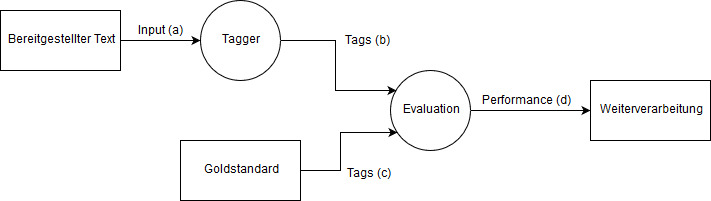
\includegraphics[width=\textwidth]{gfx/Dataflow.jpg}
	\caption{Datenfluss in einem typischen Tagging- und Evaluationsprozess}
	\label{fig:impl:plan:dataflow}
\end{figure}

Eine Übersicht hierzu bietet Abbildung \ref{fig:impl:plan:dataflow}, wobei insbesondere der Input (a) und Output (b) des Taggers interessant sind. Das Format des Goldstandards (c) ist exogen vorgegeben und das Ergebnis des Evaluationsprozesses muss lediglich RapidMiner-konform kodiert werden.

\subsection{Inputformat}
\label{sec:impl:plan:input}

Für die Eingabe an den Tagger wäre es optimal, wenn Outputs anderer Textverarbeitender RapidMiner-Erweiterungen, insbesondere vom \textit{Text Processing Plugin} :NC angenommen werden können. Hierzu kann einfach das Übergabeformat \textit{Document} aus diesem Plugin verwendet werden.

\subsection{Format für Tagger-Ergebnisse}
\label{sec:impl:plan:thru}

Abhängig vom Tagger können Ergebnisse sehr Informationsreich sein. Der LingPipe-POS-Tagger liefert beispielsweise pro Token (Wort oder Symbol) nicht nur nicht nur das aus seiner Sicht plausibelste Tag (\textit{First-Best}), sondern auch \textit{n-1} weitere, nachstehende Optionen (\textit{N-Best}), wobei \textit{n} gewählt werden kann :NC . Eine solche Menge an Metainformationen kann der Standard-Datentyp \textit{Document} seitens RapidMiner nur schwer Kodieren. Eine neu entworfene Datenstruktur, die von Operator zu Operator übergeben werden können, bietet neue Freiheiten:

\paragraph{Segmentierung} der Tag- und Token-Kette anhand von bestimmten Tags, die immer richtig erkannt werden, macht robuster gegen Verschiebungen im Ergebnis wie in Abschnitt \ref{sec:general:goals:tok} beschrieben: Wird Segment-weise verglichen und entstehen Verschiebungen durch ungleiche Token-Zerlegungen, dann verschwindet dieser Fehler, sobald ein neues Segment betreten wird, da die neuen betrachteten Segmente wieder an gleicher Stelle beginnen.
\paragraph{Anreicherung} mit Zusatzinformationen ist möglich, da im Gegensatz zu einer einfachen Textuellen Darstellung auf ein Token nicht exakt ein Tag folgen muss. Hier kann beispielsweise pro Tag eine beliebig lange Liste der \textit{N-Best} Tags stehen.

Ein solches alternatives Format ist jedoch von Operatoren, die nicht speziell dafür vorbereitet sind (wie der Evaluationsoperator), nicht lesbar. Darum müssen Ergebnisse auch immer als Typ \textit{Document} angegeben werden.

\section{Struktur}
\label{sec:impl:structure}

\subsection{Übersicht}
\label{sec:impl:structure:overview}

\begin{figure}[htb]
	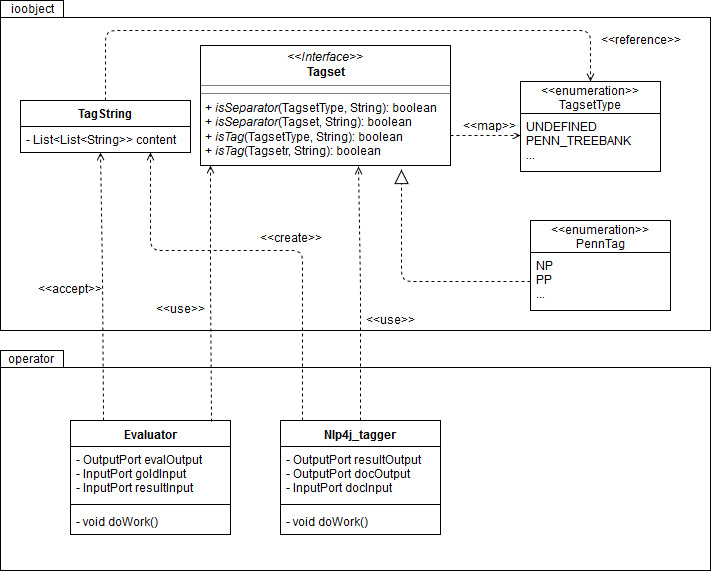
\includegraphics[width=\textwidth]{gfx/UML_Overview_simple.jpg}
	\caption{gekürztes Klassendiagramm}
	\label{fig:impl:structure:overview:uml}
\end{figure}

Abbildung \ref{fig:impl:structure:overview:uml} zeigt einen Überblick über die implementierten Klassen. Um das Diagramm überschaubar zu halten, wurden nur die Klassen eingezeichnet, die zusätzlich zum Erweiterungs-Template von RapidMiner :NC implementiert wurden. Außerdem wurden nur die notwendigen Enumerationen und Klassen für den NLP4J-Tagger aufgenommen, da andere Tagger analog strukturiert sind. Es folgt eine kurze Erklärung der verschiedenen Komponenten:

\paragraph{Operatoren:} \textit{Evaluator} und \textit{Nlp4j\_ tagger} sowie alle anderen Klassen, die von der RapidMiner-Klasse \textit{Operator} erben, sind auch in RapidMiner als Operatoren vertreten. Alle Operatoren außer Evaluator beinhalten einen POS-Tagger und überbrücken sowohl Ein- als auch Ausgangsformate zwischen dem externen RapidMiner-Modell (\textit{Document} oder \textit{TagString} ) und dem Tagging-Algorithmus selbst. Der Evaluator berechnet die Unterschiedlichkeit zwischen zwei Ergebnissen, wobei eines der beiden bestenfalls vollständig korrekt ist. :TODO

\paragraph{Tagsets:} Das Interface Tagset muss von jeder Tag-Enumeration, wie zum Beispiel dem der Penn-Treebank implementiert werden. Zusätzlich bietet es statische Methoden, die die Werte der Enumeration TagsetType auf die korrespondierenden Enumerationen abbilden, sowie Abfragen über deren Werte anbieten (hierzu wird der Typ sowie ein Tag verlangt). Die implementierenden Tagsets führen alle Part-of-Speech-Tags auf und liefern zusätzlich die Information, ob das Tag in der Datenstruktur \textit{TagString} (s.u.) Zeilen abbricht. Auf diese Weise ist es leicht, das Projekt um ein neues Set zu erweitern.

\paragraph{TagString:} Diese Klasse bietet, wie in Abschnitt \ref{sec:impl:plan:thru} angesprochen, ein einheitliches Format für POS-Tags. Sie beschreibt den Tagset-Typen sowie die Zahl an N-Besten Tags pro Token (1 für First-Best) und strukturiert die Tags in Zeilen, die immer dann enden, wenn das letzte Tag ein \textit{Separator} ist. :TODO



\section{Evaluation}
\label{sec:impl:eval}
Um Ergebnisse hinsichtlich ihrer Qualität zu prüfen, muss mit Goldstandards wie z.B. dem WSJ-Corpus :NC verglichen werden. Der Evaluationsoperator muss die Formate dieser Standards annehmen und interpretieren können. Neben dem eigentlichen Evaluieren ist also auch das \textit{Parsen} eingehender Texte eine wichtige Aufgabe des Operators. 

\subsection{Parsing}
\label{sec:impl:eval:parsing}
Verschiedene Formate kodieren POS-Tags unterschiedlich. Eine einfache Notation ist die bereits bekannte Variante, bei der nach jedem Token ein \glqq \textbackslash \grqq{} und dann das Tag folgt. Andere Notationen kodieren zusätzlich Satzstrukturinformationen, sind also mittels Klammern geschachtelt, um z.B. Teilsätze zu markieren. Hier gibt es kein Symbol, das eindeutig ein POS-Tag ankündigt. Um die Parser-Methode des Evaluationsoperators präziser arbeiten können zu lassen, wurde ein Parameter hinzugefügt, in dem man das Format wählen kann. Es wurden zwei Modi für den Parser implementiert:

\paragraph{Backslash-Notation:} In der oben genannten Notation, in der ausschließlich POS via \glqq \textbackslash \grqq{} markiert werden, ist Parsing einheitlich. Der Text wird an jedem Leerzeichen gespalten und jeder entstehende Substring am \glqq \textbackslash \grqq{}. Das POS-Tag findet sich dann im zweiten String, der bei der zweiten Spaltung entsteht.

\paragraph{"None":} Falls die Notation unbekannt ist, versucht der Parser, den Text an allen sinnvollen Symbolen, insbesondere dem Leerzeichen zu Trennen. Alle Substrings werden dann überprüft, ob sie ein POS-Tag sind. 

Zusätzlich kann die Option \textit{\glqq Ignore Brackets \grqq{}} gewählt werden, falls Klammern für die Formatierung des einzulesenden Textes verwendet wurden. diese werden dann ignoriert.
\\
Als Ergebnis gibt der Parser das Format TagString aus, das dann weiter verwendet werden kann. Der Tagset-Typ des TagStrings muss via Parameter angegeben werden.







\section{Conclusion}
\label{sec:system:conclusion}

